%%%%%%%%%%%%%%%%%%%%%%%%%%%%%%%%%%%%%%%%%
% Programming/Coding Assignment
% LaTeX Template
%
% This template has been downloaded from:
% http://www.latextemplates.com
%
% Original author:
% Ted Pavlic (http://www.tedpavlic.com)
%
% Note:
% The \lipsum[#] commands throughout this template generate dummy text
% to fill the template out. These commands should all be removed when 
% writing assignment content.
%
% This template uses a Perl script as an example snippet of code, most other
% languages are also usable. Configure them in the "CODE INCLUSION 
% CONFIGURATION" section.
%
%%%%%%%%%%%%%%%%%%%%%%%%%%%%%%%%%%%%%%%%%

%----------------------------------------------------------------------------------------
%	PACKAGES AND OTHER DOCUMENT CONFIGURATIONS
%----------------------------------------------------------------------------------------

\documentclass{article}

\usepackage{fancyhdr} % Required for custom headers
\usepackage{lastpage} % Required to determine the last page for the footer
\usepackage{extramarks} % Required for headers and footers
\usepackage[usenames,dvipsnames]{color} % Required for custom colors
\usepackage{graphicx} % Required to insert images
\usepackage{subcaption}
\usepackage{listings} % Required for insertion of code
\usepackage{courier} % Required for the courier font
\usepackage{lipsum} % Used for inserting dummy 'Lorem ipsum' text into the template
\usepackage{hyperref} % Used for linking to websites
\usepackage{amsmath, amsthm, amssymb} % Required for writing equations
\usepackage{pythonhighlight} % Required for including Python code
\usepackage{siunitx} % Required for scientific notation
\usepackage{multicol}


% Margins
\topmargin=-0.45in
\evensidemargin=0in
\oddsidemargin=0in
\textwidth=6.5in
\textheight=9.0in
\headsep=0.25in

\linespread{1.1} % Line spacing

% Set up the header and footer
\pagestyle{fancy}
\lhead{\hmwkFirstAuthorName, \hmwkSecondAuthorName} % Top left header
\chead{\hmwkClass\ (\hmwkClassTime): \hmwkTitle} % Top center head
%\rhead{\firstxmark} % Top right header
\lfoot{\lastxmark} % Bottom left footer
\cfoot{} % Bottom center footer
\rfoot{Page\ \thepage\ of\ \protect\pageref{LastPage}} % Bottom right footer
\renewcommand\headrulewidth{0.4pt} % Size of the header rule
\renewcommand\footrulewidth{0.4pt} % Size of the footer rule

\setlength\parindent{0pt} % Removes all indentation from paragraphs

%----------------------------------------------------------------------------------------
%	CODE INCLUSION CONFIGURATION
%----------------------------------------------------------------------------------------

\definecolor{MyDarkGreen}{rgb}{0.0,0.4,0.0} % This is the color used for comments
\lstloadlanguages{Perl} % Load Perl syntax for listings, for a list of other languages supported see: ftp://ftp.tex.ac.uk/tex-archive/macros/latex/contrib/listings/listings.pdf
\lstset{language=Perl, % Use Perl in this example
	frame=single, % Single frame around code
	basicstyle=\small\ttfamily, % Use small true type font
	keywordstyle=[1]\color{Blue}\bf, % Perl functions bold and blue
	keywordstyle=[2]\color{Purple}, % Perl function arguments purple
	keywordstyle=[3]\color{Blue}\underbar, % Custom functions underlined and blue
	identifierstyle=, % Nothing special about identifiers                                         
	commentstyle=\usefont{T1}{pcr}{m}{sl}\color{MyDarkGreen}\small, % Comments small dark green courier font
	stringstyle=\color{Purple}, % Strings are purple
	showstringspaces=false, % Don't put marks in string spaces
	tabsize=5, % 5 spaces per tab
	%
	% Put standard Perl functions not included in the default language here
	morekeywords={rand},
	%
	% Put Perl function parameters here
	morekeywords=[2]{on, off, interp},
	%
	% Put user defined functions here
	morekeywords=[3]{test},
	%
	morecomment=[l][\color{Blue}]{...}, % Line continuation (...) like blue comment
	numbers=left, % Line numbers on left
	firstnumber=1, % Line numbers start with line 1
	numberstyle=\tiny\color{Blue}, % Line numbers are blue and small
	stepnumber=5 % Line numbers go in steps of 5
}

% Creates a new command to include a perl script, the first parameter is the filename of the script (without .pl), the second parameter is the caption
\newcommand{\perlscript}[2]{
	\begin{itemize}
		\item[]\lstinputlisting[caption=#2,label=#1]{#1.pl}
	\end{itemize}
}

%----------------------------------------------------------------------------------------
%	DOCUMENT STRUCTURE COMMANDS
%	Skip this unless you know what you're doing
%----------------------------------------------------------------------------------------

% Header and footer for when a page split occurs within a problem environment
\newcommand{\enterProblemHeader}[1]{
	%\nobreak\extramarks{#1}{#1 continued on next page\ldots}\nobreak
	%\nobreak\extramarks{#1 (continued)}{#1 continued on next page\ldots}\nobreak
}

% Header and footer for when a page split occurs between problem environments
\newcommand{\exitProblemHeader}[1]{
	%\nobreak\extramarks{#1 (continued)}{#1 continued on next page\ldots}\nobreak
	%\nobreak\extramarks{#1}{}\nobreak
}

\setcounter{secnumdepth}{0} % Removes default section numbers
\newcounter{homeworkProblemCounter} % Creates a counter to keep track of the number of problems
\setcounter{homeworkProblemCounter}{0}

\newcommand{\homeworkProblemName}{}
\newenvironment{homeworkProblem}[1][Part \arabic{homeworkProblemCounter}]{ % Makes a new environment called homeworkProblem which takes 1 argument (custom name) but the default is "Problem #"
	\stepcounter{homeworkProblemCounter} % Increase counter for number of problems
	\renewcommand{\homeworkProblemName}{#1} % Assign \homeworkProblemName the name of the problem
	\section{\homeworkProblemName} % Make a section in the document with the custom problem count
	\enterProblemHeader{\homeworkProblemName} % Header and footer within the environment
}{
	\exitProblemHeader{\homeworkProblemName} % Header and footer after the environment
}

\newcommand{\problemAnswer}[1]{ % Defines the problem answer command with the content as the only argument
	\noindent\framebox[\columnwidth][c]{\begin{minipage}{0.98\columnwidth}#1\end{minipage}} % Makes the box around the problem answer and puts the content inside
}

\newcommand{\homeworkSectionName}{}
\newenvironment{homeworkSection}[1]{ % New environment for sections within homework problems, takes 1 argument - the name of the section
	\renewcommand{\homeworkSectionName}{#1} % Assign \homeworkSectionName to the name of the section from the environment argument
	\subsection{\homeworkSectionName} % Make a subsection with the custom name of the subsection
	\enterProblemHeader{\homeworkProblemName\ [\homeworkSectionName]} % Header and footer within the environment
}{
	\enterProblemHeader{\homeworkProblemName} % Header and footer after the environment
}

%----------------------------------------------------------------------------------------
%	NAME AND CLASS SECTION
%----------------------------------------------------------------------------------------

\newcommand{\hmwkTitle}{Project\ \#4 \\ Tic-Tac-Toe with Policy Gradient} % Assignment title
\newcommand{\hmwkDueDate}{Monday,\ March\ 19,\ 2018} % Due date
\newcommand{\hmwkClass}{CSC411} % Course/class
\newcommand{\hmwkClassTime}{L2501} % Class/lecture time
\newcommand{\hmwkFirstAuthorName}{Dhruv Chawla} % First name
\newcommand{\hmwkSecondAuthorName}{Saila Maham Shama } % First name

%----------------------------------------------------------------------------------------
%	TITLE PAGE
%----------------------------------------------------------------------------------------

\title{
	\vspace{2in}
	\textmd{\textbf{\hmwkClass:\ \hmwkTitle}}\\
	\normalsize\vspace{0.1in}\small{Due\ on\ \hmwkDueDate}\\
	\vspace{0.1in}
	\vspace{3in}
}

\author{\textbf{\hmwkFirstAuthorName, \hmwkSecondAuthorName}}
%\date{} % Insert date here if you want it to appear below your name

%----------------------------------------------------------------------------------------

\begin{document}

\maketitle
\clearpage
%----------------------------------------------------------------------------------------
%	PROBLEM 1
%----------------------------------------------------------------------------------------

% To have just one problem per page, simply put a \clearpage after each problem

\begin{homeworkProblem}

\noindent \textit{Tic-Tac-Toe text output}
\begin{verbatim}


>>> env.render()
...
...
...
====
>>> env.step(4)
(array([0, 0, 0, 0, 1, 0, 0, 0, 0]), 'valid', False)
>>> env.render()
...
.x.
...
====
>>> env.step(1)
(array([0, 2, 0, 0, 1, 0, 0, 0, 0]), 'valid', False)
>>> env.render()
.o.
.x.
...
====
>>> env.step(0)
>>> env.step(2)
(array([1, 2, 2, 0, 1, 0, 0, 0, 0]), 'valid', False)
>>> env.render()
xoo
.x.
...
====
>>> env.step(8)
(array([1, 2, 2, 0, 1, 0, 0, 0, 1]), 'win', True)
>>> env.render()
xoo
.x.
..x
====
\end{verbatim}

\end{homeworkProblem}
\clearpage
%----------------------------------------------------------------------------------------
%	PROBLEM 2
%----------------------------------------------------------------------------------------

\begin{homeworkProblem}

\subsection*{2(a)}
\begin{python}

class Policy(nn.Module):
"""
The Tic-Tac-Toe Policy
"""
def __init__(self, input_size=27, hidden_size=64, output_size=9):
	super(Policy, self).__init__()
	self.fc1 = nn.Linear(input_size, hidden_size)
	self.fc2 = nn.Linear(hidden_size, output_size)

def forward(self, x):
	x = F.relu(self.fc1(x))
	x = self.fc2(x)
	softmax = nn.Softmax()
	return softmax(x)	
\end{python}

\subsection*{2(b)}

Running the following script
\begin{python}
	policy = Policy()
		
	# xoo
	# .x.
	# ..x
	# =====
	
	state = np.array([1, 2, 2, 0, 1, 0, 0, 0, 1)]	
	
	state = torch.from_numpy(state).long().unsqueeze(0)
	state = torch.zeros(3,9).scatter_(0,state,1).view(1,27)
	print(state)
\end{python}
we yield the output
\begin{verbatim}
	Columns 0 to 12 
	0     0     0     1     0     1     1     1     0     1     0     0     0
	
	Columns 13 to 25 
	1     0     0     0     1     0     1     1     0     0     0     0     0
	
	Columns 26 to 26 
	0
	[torch.FloatTensor of size 1x27]
\end{verbatim}

The output seems to imply that the first nine dimensions indicat entries that are empty, the second nine dimensions indicate entries that are x's and the last nine dimensions indicate entires that are o's. 


\subsection*{2(c)}
The output of the select$\_$output function is a nine-dimensional vector indicates which position of the tic-tac-toe table to place that player's mark. The policy is stochastic. 

\end{homeworkProblem}


\clearpage
%----------------------------------------------------------------------------------------
%%	PROBLEM 3
%%----------------------------------------------------------------------------------------

\begin{homeworkProblem}
	
\subsection{3(a)}
\begin{python}

def compute_returns(rewards, gamma=1.0):
"""
Compute returns for each time step, given the rewards
@param rewards: list of floats, where rewards[t] is the reward
obtained at time step t
@param gamma: the discount factor
@returns list of floats representing the episode's returns
G_t = r_t + \gamma r_{t+1} + \gamma^2 r_{t+2} + ..
"""
	G = [0] * len(rewards)
	
	for i in range(len(rewards)-1, -1, -1):
	if i == len(rewards)-1: G[i] = rewards[i]
	else: G[i] = rewards[i] + gamma * G[i+1]
	
	return G	
\end{python}

\subsection*{3(b)}
We cannot update the weights in the middle of an episode because s

\end{homeworkProblem}
\clearpage

%----------------------------------------------------------------------------------------
%	PROBLEM 4
%----------------------------------------------------------------------------------------

\begin{homeworkProblem}
\subsection*{4(a)}

The modified \texttt{get\_reward(status)} function is included below:\\

\begin{python}
def get_reward(status):
    """Returns a numeric given an environment status."""
    return {
            Environment.STATUS_VALID_MOVE  : 1,
            Environment.STATUS_INVALID_MOVE: -250,
            Environment.STATUS_WIN         : 500,
            Environment.STATUS_TIE         : -3,
            Environment.STATUS_LOSE        : -3
    }[status]
\end{python}


\subsection*{4(b)}

There are positive and negative rewards. Negative rewards are given for undesirable outcomes (invalid move, tie and lose) while positive rewards are given for winning and making a valid move. Initially the reward for tie was positive and comparable to the reward for winning but was then made negative to increase the win rate (we observed that the AI was going for ties and was effectively treating tie-ing the same as winning).\\

As far as the magnitude of the rewards go, the reward for winning was increased by a factor of 100 compared to the magnitudes of losing and tieing to incentivize the AI to win more. The reward for making an invalid move was initially -1 but was increased in magnitude to bring down the number of invalid moves during the game.\\

\end{homeworkProblem}
\clearpage

%----------------------------------------------------------------------------------------
%	PROBLEM 5
%----------------------------------------------------------------------------------------

\begin{homeworkProblem}
%changing hyperparameters? 
\subsection*{5(a)}
\begin{figure}[h]
	\caption{Training curve ($\#$ hidden units: 64)}
	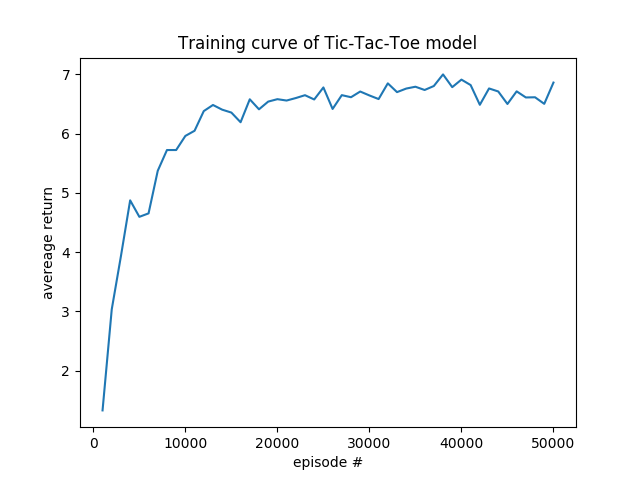
\includegraphics[width=\linewidth]{figures/part5a.png}
	\label{fig:part5a}
\end{figure}
\subsection*{5(b)}
The number of hidden units were reset to values 32, 128 and 256 to obtain the following training curves:

\newpage
\begin{figure}[h]
	\caption{Training curve ($\#$ hidden units: 32)}
	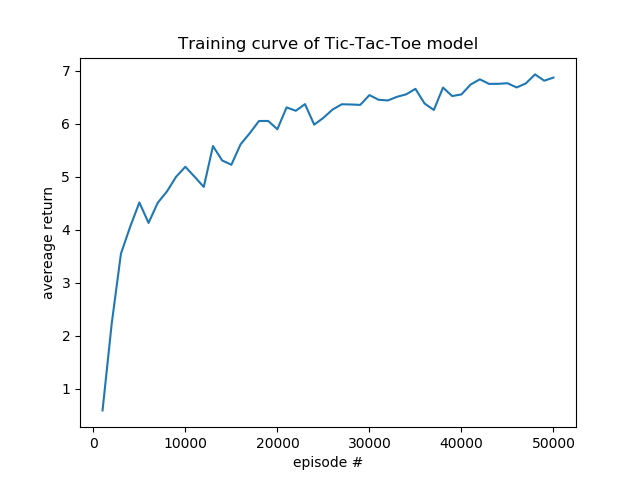
\includegraphics[width=\linewidth]{figures/part5b_32.png}
	\label{fig:part5b_32}
\end{figure}
\newpage

\begin{figure}[h]
	\caption{Training curve ($\#$ hidden units: 128)}
	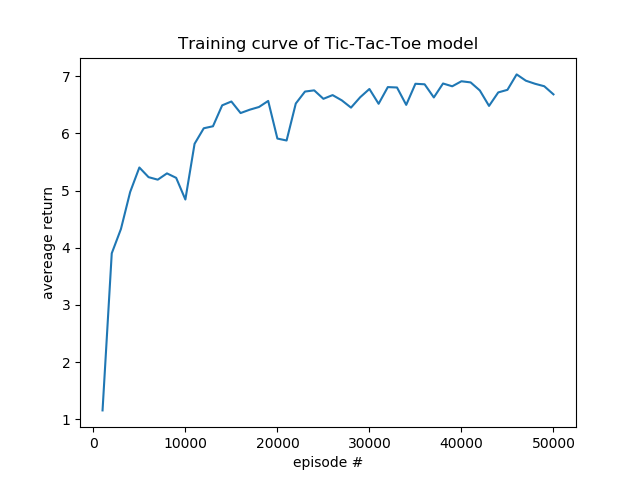
\includegraphics[width=\linewidth]{figures/part5b_128.png}
	\label{fig:part5b_128}

\end{figure}
\newpage
\begin{figure}[h]
	\caption{Training curve ($\#$ hidden units: 256)}
	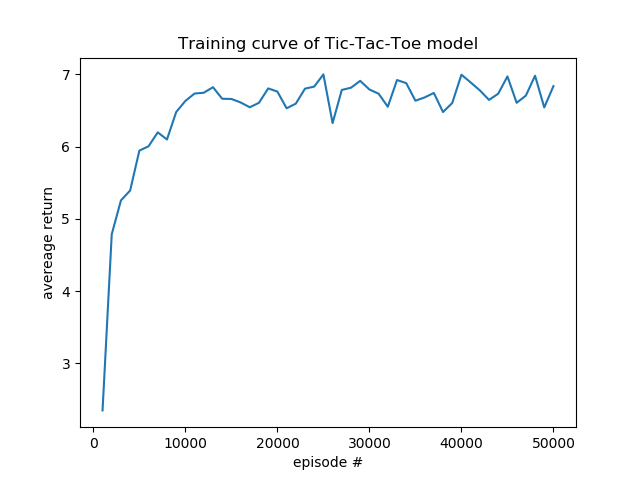
\includegraphics[width=\linewidth]{figures/part5b_256.png}
	\label{fig:part5b_256}
\end{figure}
\newpage

\subsection*{5(c)}
From Figure \ref{fig:part5a}, it seems as though the policy never played invalid moves. 

\subsection*{5(d)}
Using the final learned policy, the agent wins 98/100 games and ties 2/100. This can be seen in Figure \ref{fig:part6}. Five of the 100 sample games are displayed below:

\begin{multicols}{5}
	\begin{verbatim}
	Game: 0
	..x
	...
	o..
	====
	o.x
	...
	o.x
	====
	o.x
	..x
	o.x
	====
	\end{verbatim}
	\columnbreak
	\begin{verbatim}
	Game: 19
	o.x
	...
	...
	====
	o.x
	o..
	..x
	====
	o.x
	o.x
	..x
	====
	\end{verbatim}
	\columnbreak
%	\begin{verbatim}
%	Game: 38
%	..x
%	..o
%	...
%	====
%	..x
%	.xo
%	..o
%	====
%	..x
%	.xo
%	x.o
%	====
%	\end{verbatim}
%	\columnbreak
	\begin{verbatim}
	Game: 57
	..x
	o..
	...
	====
	o.x
	o..
	..x
	====
	o.x
	o.x
	..x
	====
	\end{verbatim}
	\columnbreak
	\begin{verbatim}
	Game: 76
	.ox
	...
	...
	====
	.ox
	...
	.ox
	====
	.ox
	..x
	.ox
	====
	\end{verbatim}
	\columnbreak
	\begin{verbatim}
	Game: 95
	..x
	...
	..o
	====
	.ox
	.x.
	..o
	====
	.ox
	.x.
	x.o
	====
	\end{verbatim}
	\columnbreak
\end{multicols}
\newpage
\end{homeworkProblem}

\clearpage

%----------------------------------------------------------------------------------------
%	PROBLEM 6
%----------------------------------------------------------------------------------------
\begin{homeworkProblem}
Refer to Figure \ref{fig:part6}.
\begin{figure}[h]
	\caption{}
	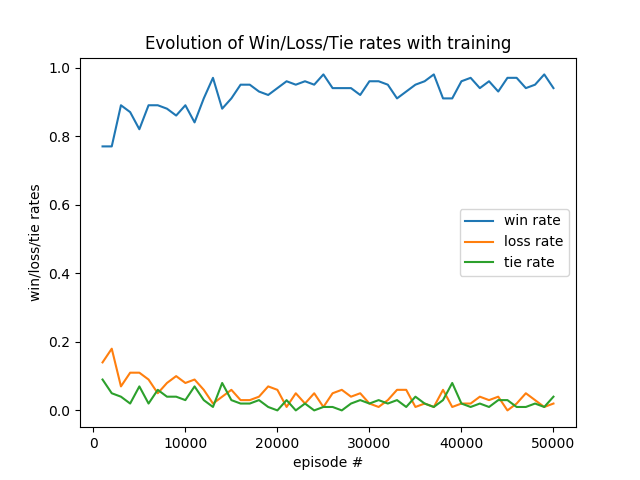
\includegraphics[width=\linewidth]{figures/part6.png}
	\label{fig:part6}
\end{figure}

\end{homeworkProblem}
\clearpage
%----------------------------------------------------------------------------------------
%	PROBLEM 7
%----------------------------------------------------------------------------------------
\begin{homeworkProblem}
	Refer to Figure \ref{fig:part7}.
	\begin{figure}[h]
		\centering
		\caption{Evolution of first move probability for each of the 9 cells of the tic-tac-toe board}
		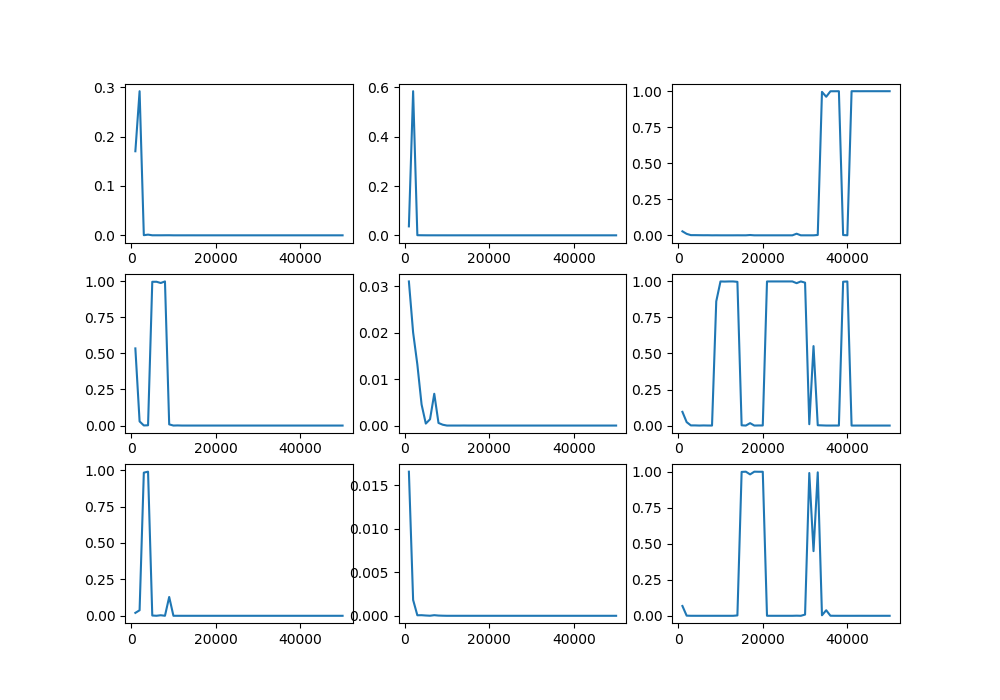
\includegraphics[width=\linewidth]{figures/part7.png}
		\label{fig:part7}
	\end{figure}
	
\end{homeworkProblem}
\clearpage

%----------------------------------------------------------------------------------------
%	PROBLEM 8
%----------------------------------------------------------------------------------------
\begin{homeworkProblem}
\end{homeworkProblem}





%----------------------------------------------------------------------------------------

\end{document}